\documentclass[12pt,oneside]{article}

\usepackage[russian]{babel}
\usepackage[utf8]{inputenc}
\usepackage{amsmath}
\usepackage{amssymb}
\usepackage{graphicx}
\usepackage{multicol}
\usepackage[14pt]{extsizes}
\usepackage[linesnumbered,boxed]{algorithm2e}
\usepackage{amsthm}
\usepackage{listings}
\usepackage{epstopdf}


\binoppenalty = 10000
\relpenalty = 10000
\textheight = 23cm
\textwidth = 17cm
\oddsidemargin = 0pt
\topmargin = -1.5cm
\parskip = 0pt
\tolerance = 2000
\flushbottom

\pagestyle{myheadings}

\begin{document}

\section{Эксперименты на infinite cluttered MNIST}

\subsection{Сравнение для Adam}

\begin{figure}[h!]
\centering
\begin{minipage}{0.45\textwidth}
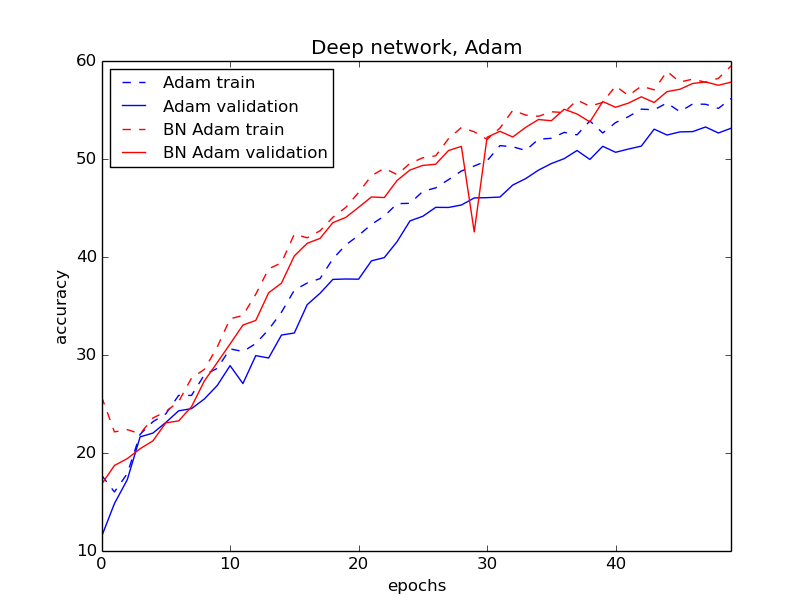
\includegraphics[scale=0.45]{images/clDeep_adam.png}
\end{minipage} \hfill
\begin{minipage}{0.45\textwidth}
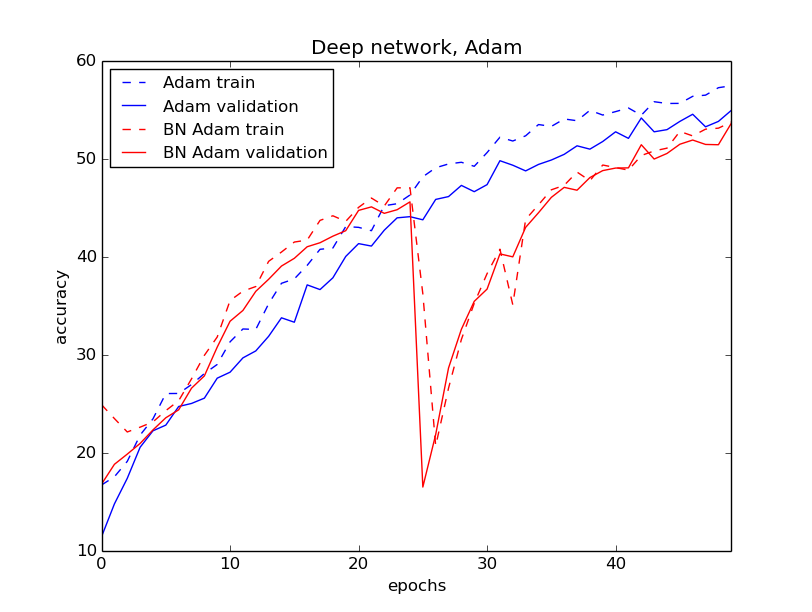
\includegraphics[scale=0.45]{images/clDeep_adam2.png}
\end{minipage}
\caption{\small Глубокая сеть ($10$ HL $\times 100$)}
\end{figure}


\begin{figure}[h!]
\centering
\begin{minipage}{0.45\textwidth}
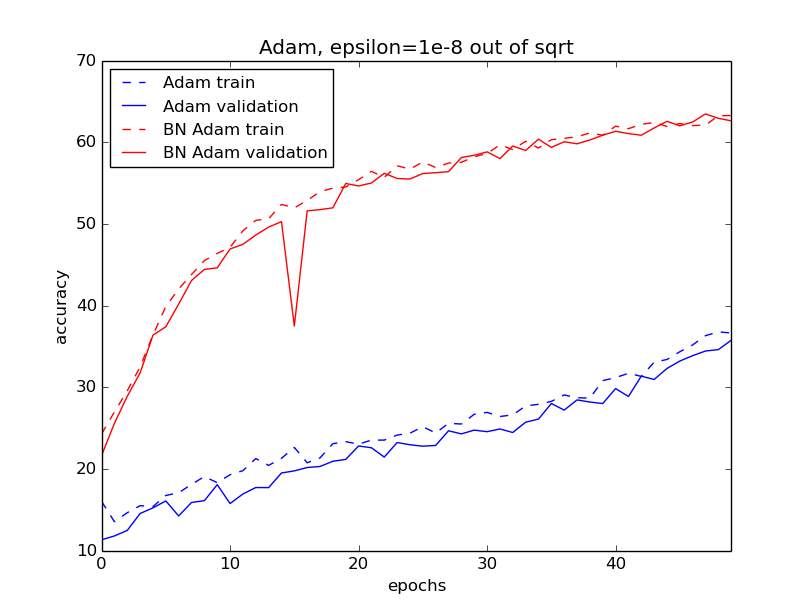
\includegraphics[scale=0.45]{images/clAdam1.png}
\end{minipage} \hfill
\begin{minipage}{0.45\textwidth}
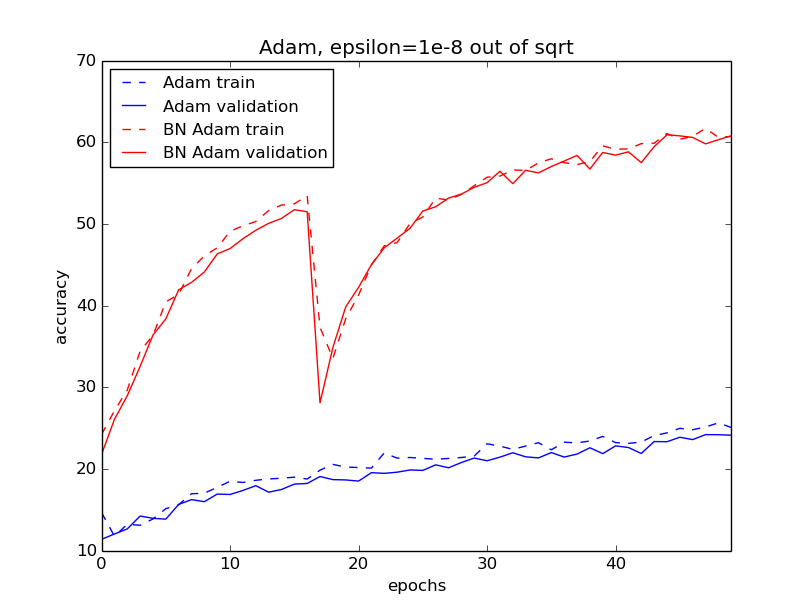
\includegraphics[scale=0.45]{images/clAdam1_s10.png}
\end{minipage}
\caption{\small $\epsilon = 10^{-8}$ вне корня ($3$ HL $\times 100$)}
\end{figure}

\newpage

\begin{figure}[h!]
\centering
\begin{minipage}{0.45\textwidth}
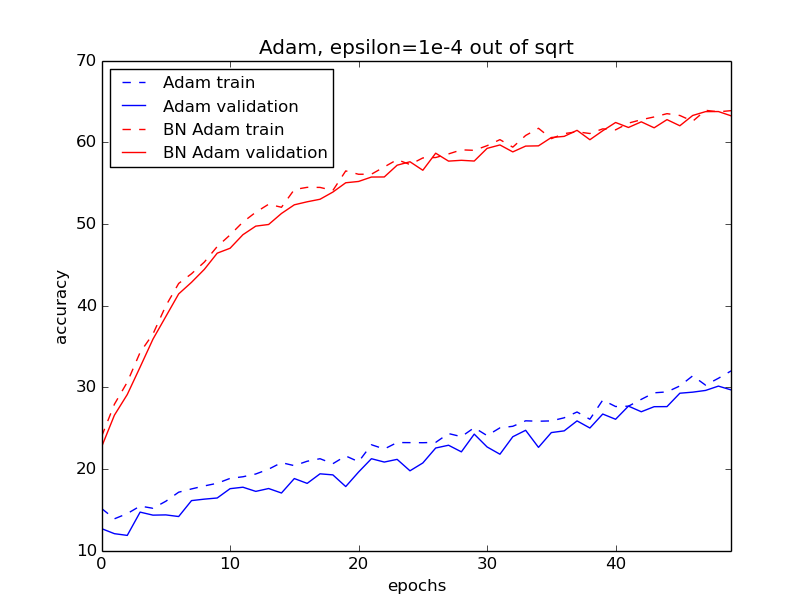
\includegraphics[scale=0.45]{images/clAdam2.png}
\end{minipage} \hfill
\begin{minipage}{0.45\textwidth}
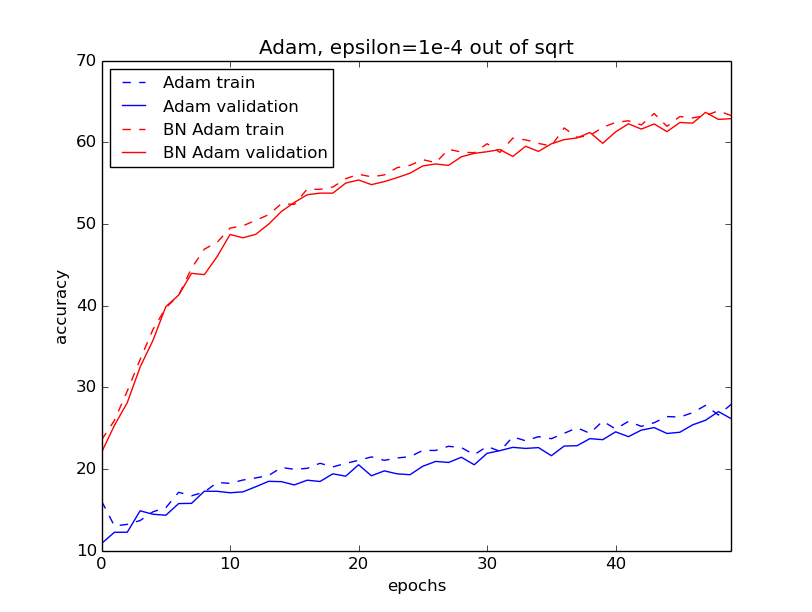
\includegraphics[scale=0.45]{images/clAdam2_s10.png}
\end{minipage}
\caption{\small $\epsilon = 10^{-4}$ вне корня ($3$ HL $\times 100$)}
\end{figure}

\begin{figure}[h!]
\centering
\begin{minipage}{0.45\textwidth}
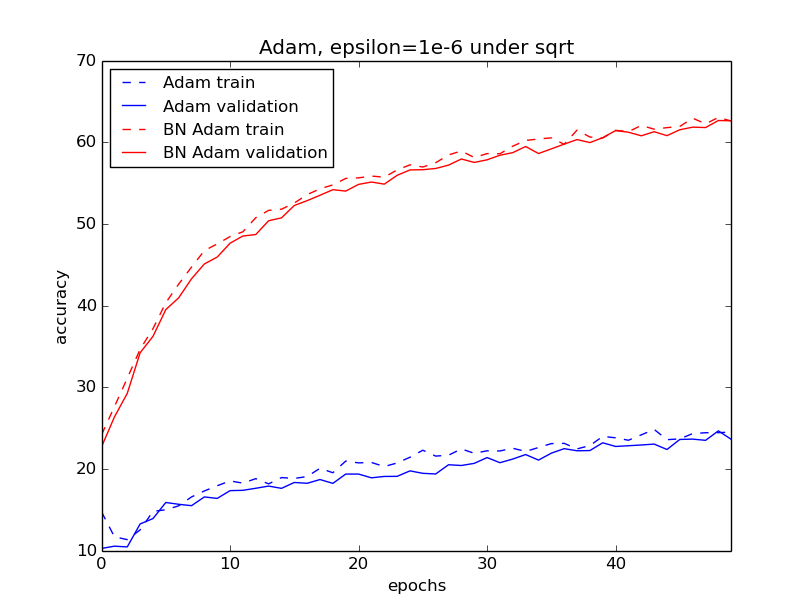
\includegraphics[scale=0.45]{images/clAdam3.png}
\end{minipage} \hfill
\begin{minipage}{0.45\textwidth}
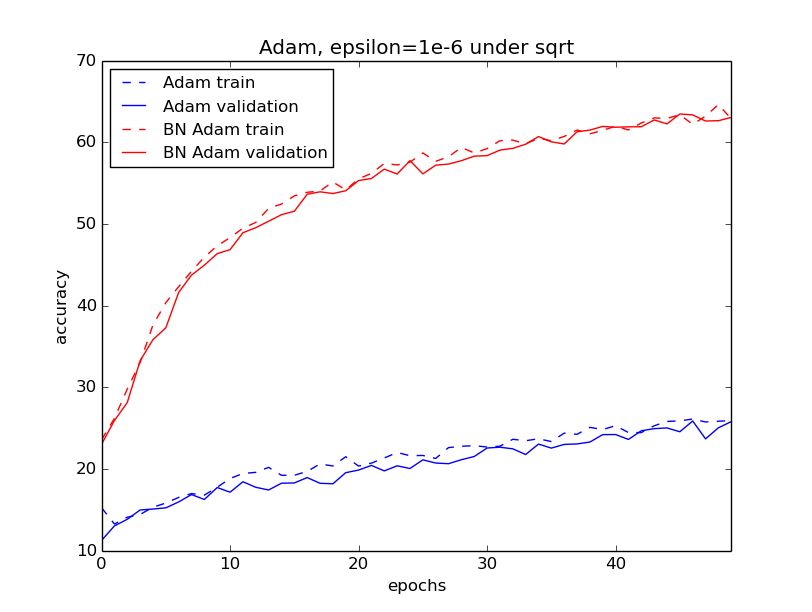
\includegraphics[scale=0.45]{images/clAdam3_s10.png}
\end{minipage}
\caption{\small $\epsilon = 10^{-6}$ под корнем, как сделано в других методах ($3$ HL $\times 100$)}
\end{figure}

Делаем выводы, что 

\begin{enumerate}
\item батч-нормализация может сильно прыгать при дефолтных параметрах метода;
\item батч-нормализация перестает прыгать, если увеличить эпсилон;
\item на неглубокой сети (3 скрытых слоя) Адам не успевает обучиться из-за сложной выборки и малого количества параметров;
\item на сети с 10 скрытыми слоями батч-нормализация слабо улучшает Адам.
\end{enumerate}

\newpage

\subsection{Остальные методы}

\begin{figure}[h!]
\centering
\begin{minipage}{0.45\textwidth}
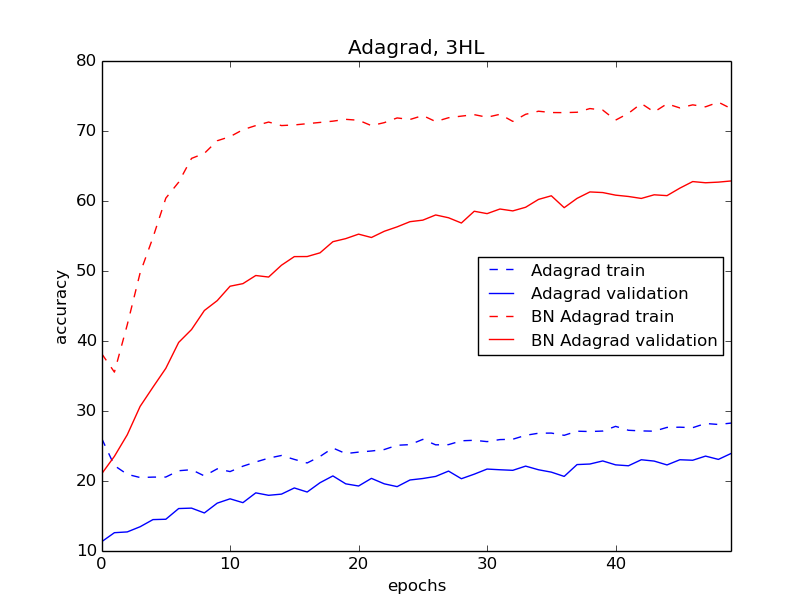
\includegraphics[scale=0.38]{images/clAdagrad.png}
\caption{\small Adagrad, $3$ HL $\times 100$}
\end{minipage} \hfill
\begin{minipage}{0.45\textwidth}
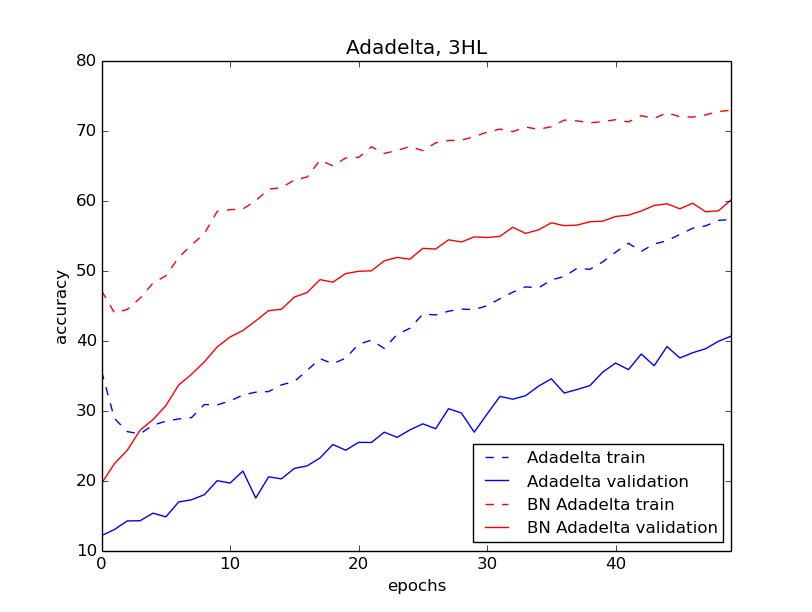
\includegraphics[scale=0.38]{images/clAdadelta.png}
\caption{\small Adadelta, $3$ HL $\times 100$}
\end{minipage} \vfill
\begin{minipage}{0.45\textwidth}
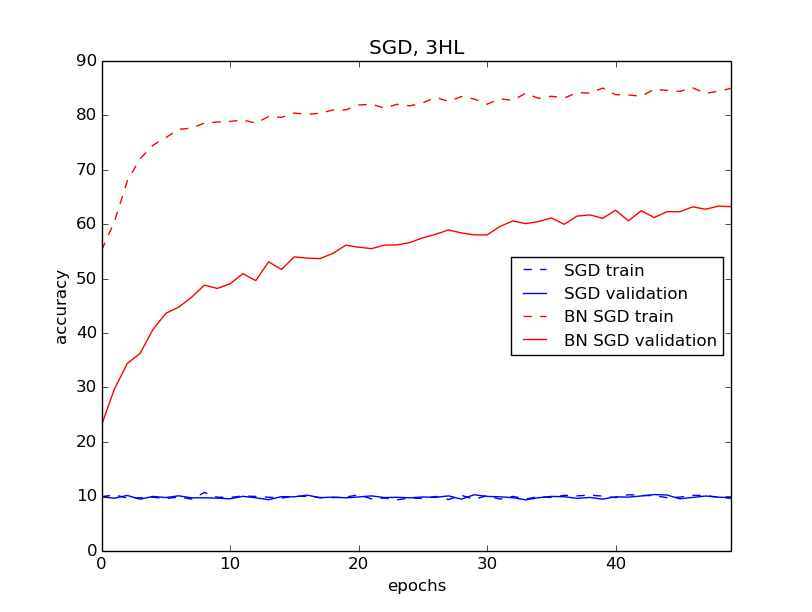
\includegraphics[scale=0.38]{images/clSgd.png}
\caption{\small SGD, $3$ HL $\times 100$}
\end{minipage} \hfill
\begin{minipage}{0.45\textwidth}
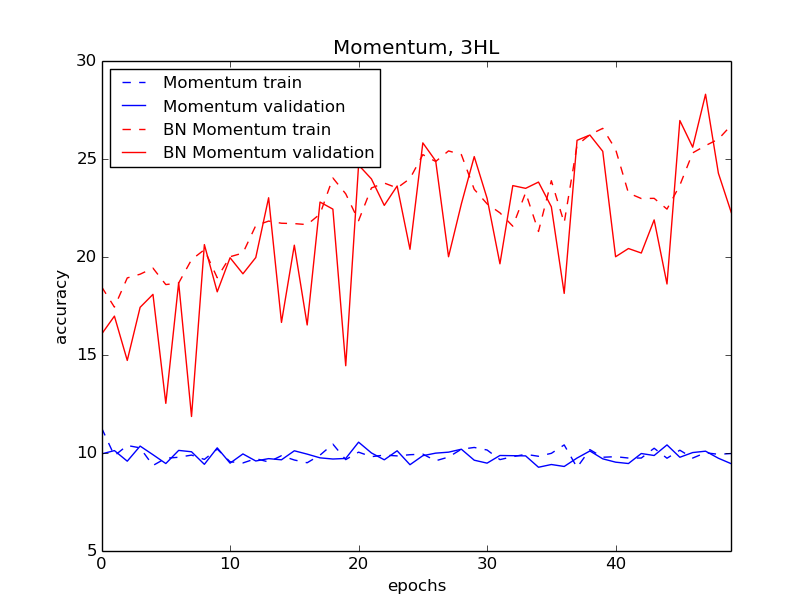
\includegraphics[scale=0.38]{images/clMomentum.png}
\caption{\small Momentum, $3$ HL $\times 100$}
\end{minipage}
\begin{minipage}{0.45\textwidth}
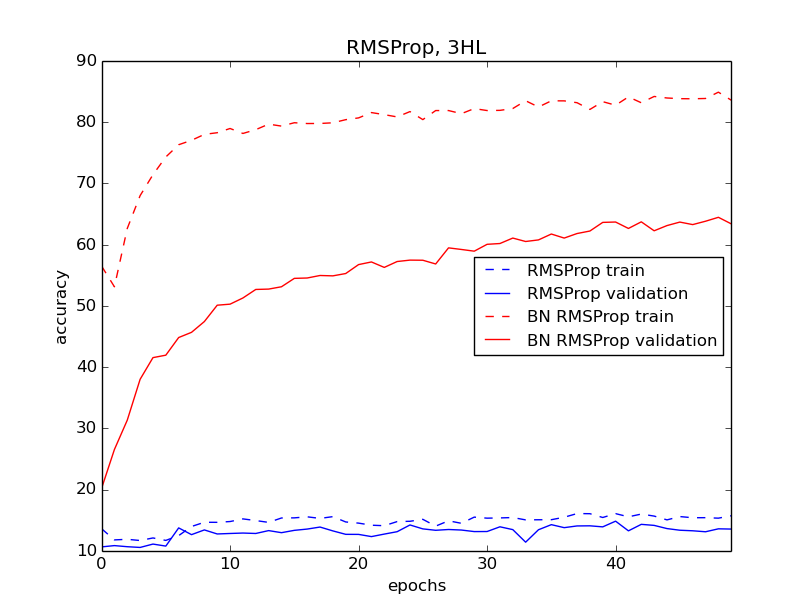
\includegraphics[scale=0.38]{images/clRmsprop.png}
\caption{\small RMSProp, $3$ HL $\times 100$}
\end{minipage}
\end{figure}

\newpage

Выводы:

\begin{enumerate}
\item рейт здесь особо не подбирался, поэтому нужно дополнительное исследование;
\item моментум сильно скачет, хотя рейт у них с SGD выставлен одинаковый;
\item моментум -- единственный метод, для которого батч-нормализация на тренировочной и валидационной выборках почти не различается;
\end{enumerate}

\newpage

\section{Эксперименты на MNIST}

\subsection{Сравнение для Adam}

\begin{figure}[h!]
\centering
\begin{minipage}{0.45\textwidth}
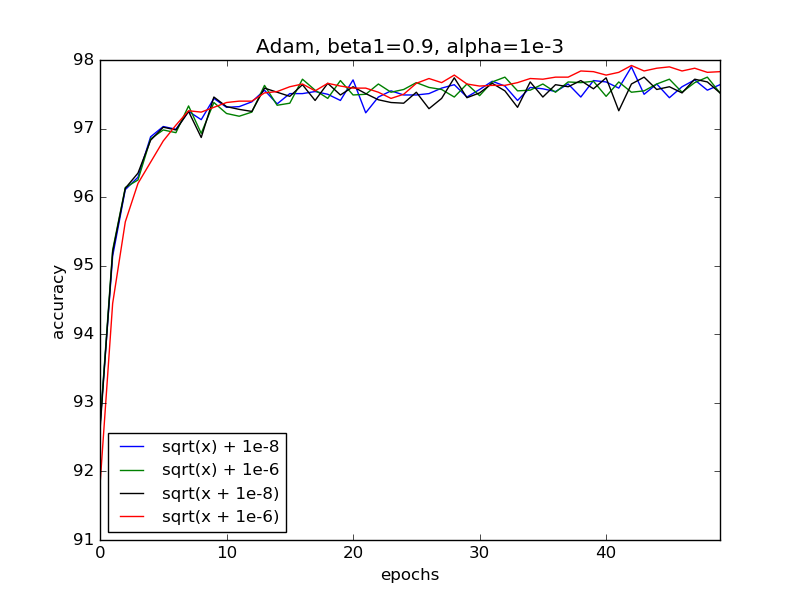
\includegraphics[scale=0.45]{images/mnistEpsilon.png}
\caption{\small Различные эпсилон-стратегии}
\end{minipage} \hfill
\begin{minipage}{0.45\textwidth}
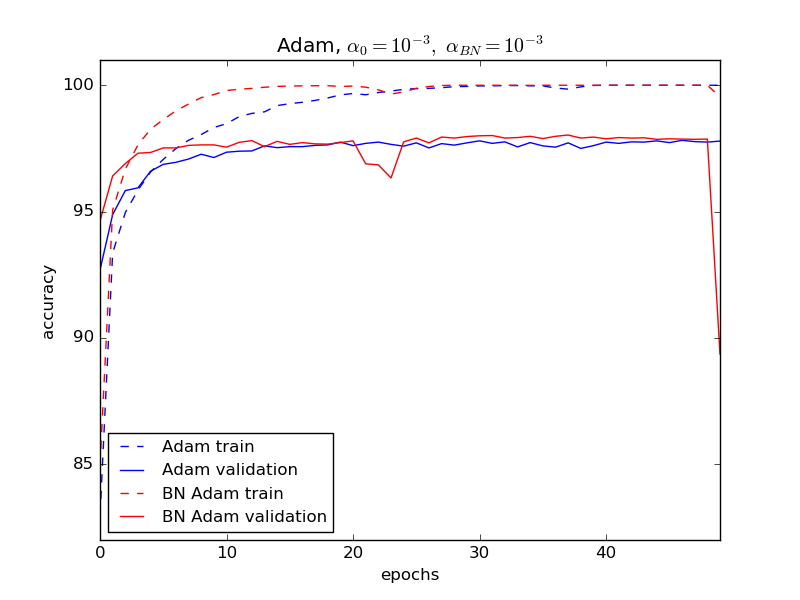
\includegraphics[scale=0.45]{images/mnistAdam1.png}
\caption{\small Адам, $3$ HL $\times 100$}
\end{minipage} \vfill
\begin{minipage}{0.45\textwidth}
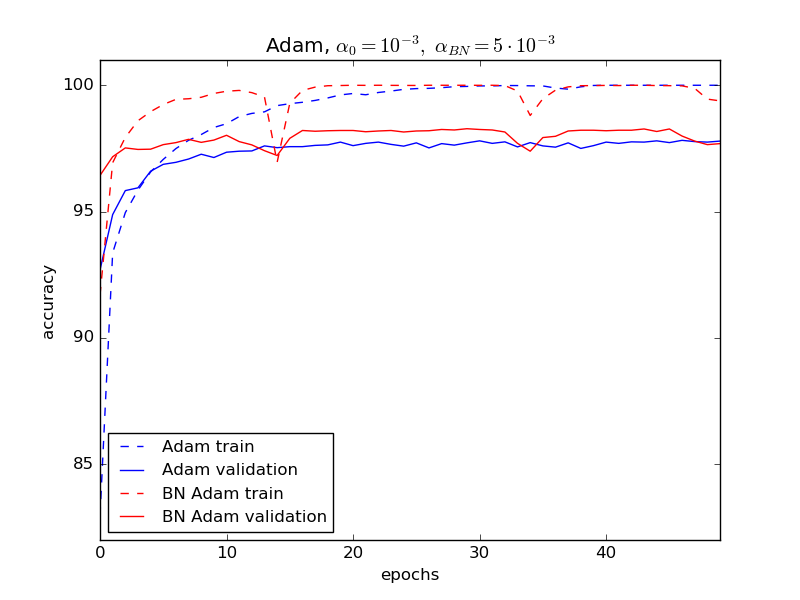
\includegraphics[scale=0.45]{images/mnistAdam2.png}
\caption{\small Адам, $3$ HL $\times 100$}
\end{minipage} \hfill
\begin{minipage}{0.45\textwidth}
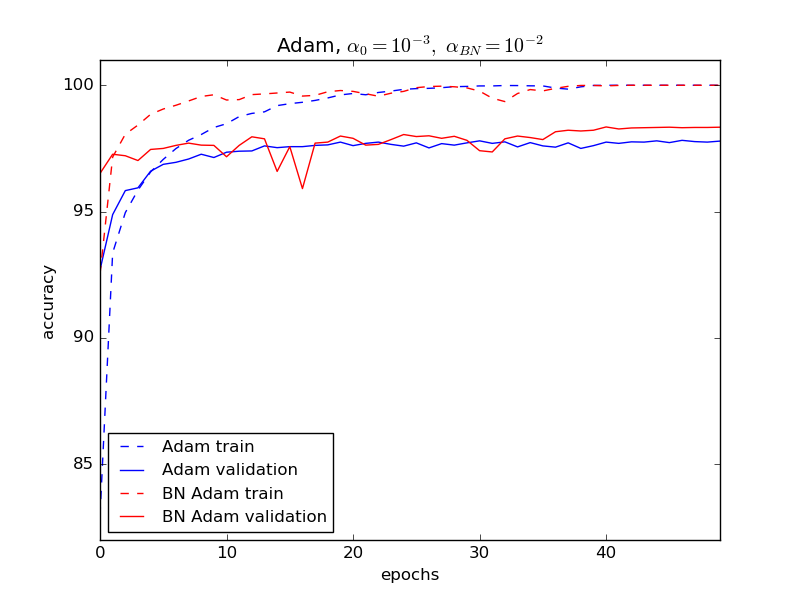
\includegraphics[scale=0.45]{images/mnistAdam3.png}
\caption{\small Адам, $3$ HL $\times 100$}
\end{minipage}
\end{figure}

\newpage

\begin{figure}[h!]
\centering
\begin{minipage}{0.45\textwidth}
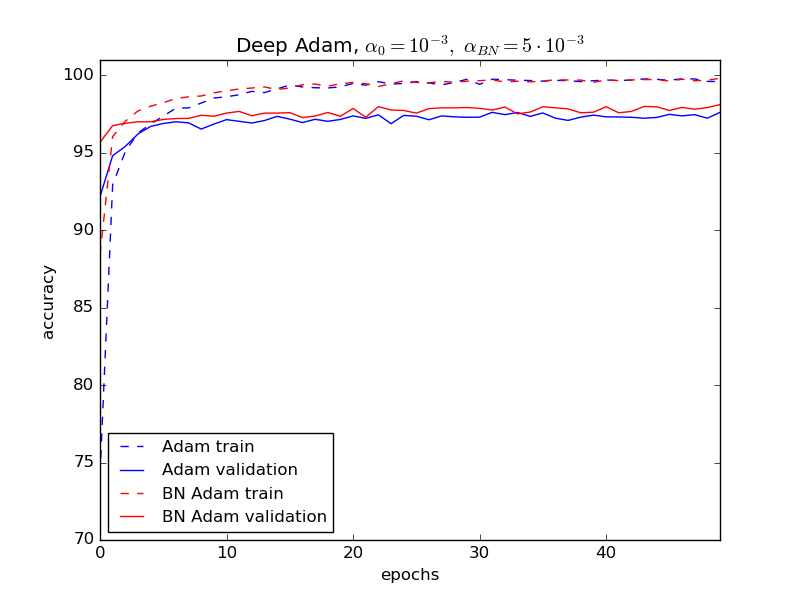
\includegraphics[scale=0.45]{images/mnistDeepAdam1.png}
\caption{\small Адам на глубокой сети, $10$ HL $\times 100$}
\end{minipage} \hfill
\begin{minipage}{0.45\textwidth}
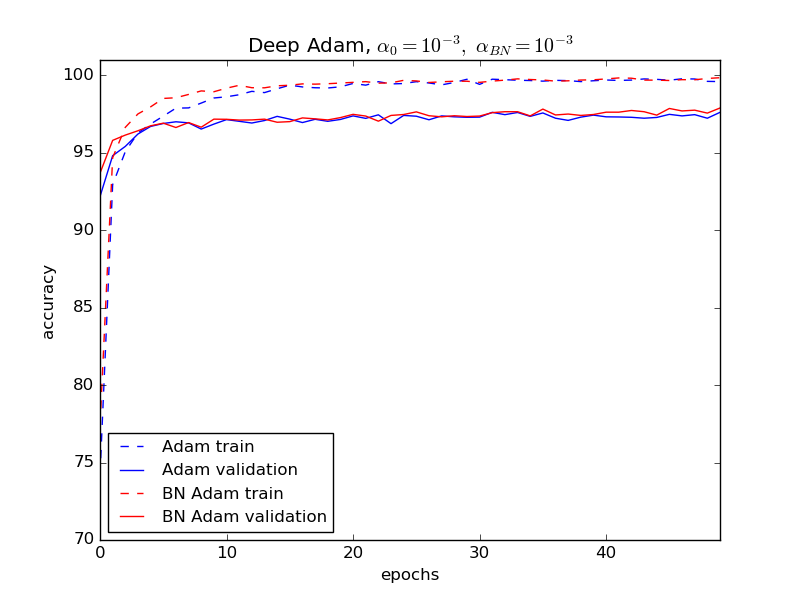
\includegraphics[scale=0.45]{images/mnistDeepAdam2.png}
\caption{\small Адам на глубокой сети, $10$ HL $\times 100$}
\end{minipage}
\end{figure}


\newpage
\subsection{Остальне методы}

\begin{figure}[h!]
\centering
\begin{minipage}{0.45\textwidth}
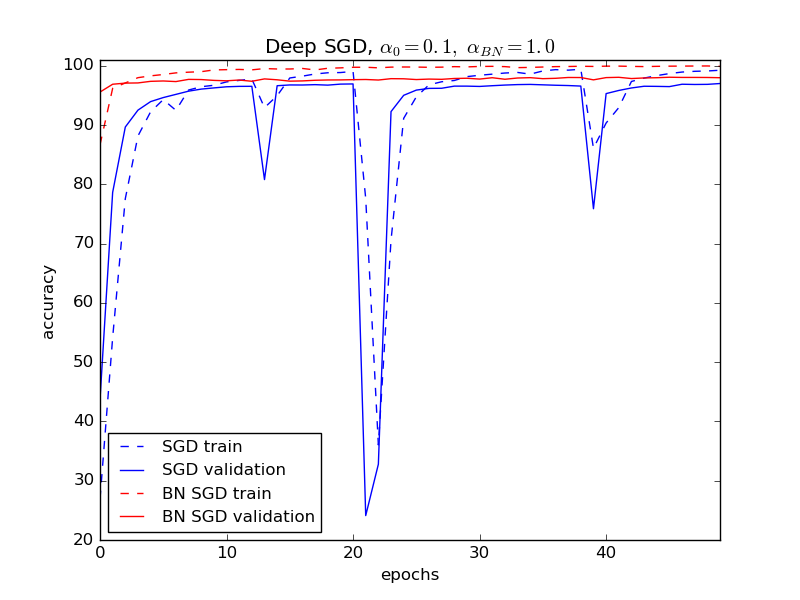
\includegraphics[scale=0.45]{images/mnistDeepSGD1.png}
\caption{\small SGD на глубокой сети, $10$ HL $\times 100$}
\end{minipage} \hfill
\begin{minipage}{0.45\textwidth}
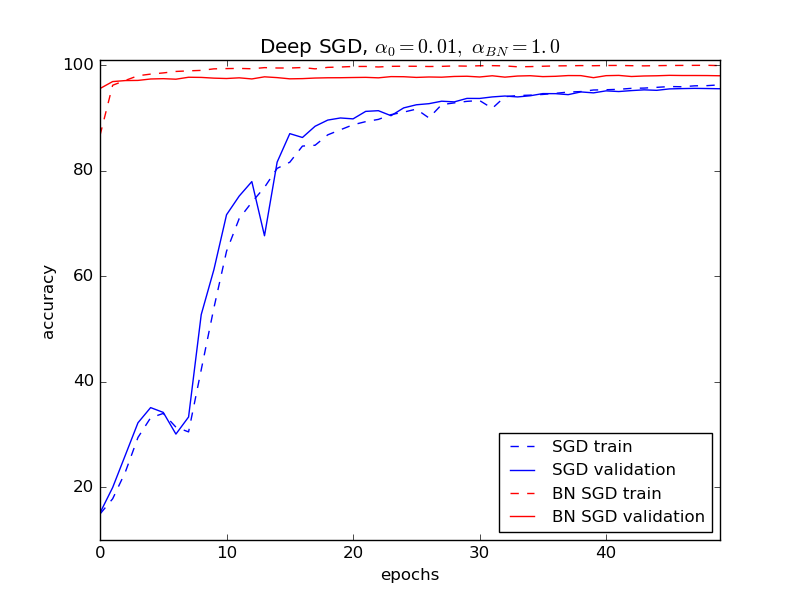
\includegraphics[scale=0.45]{images/mnistDeepSGD2.png}
\caption{\small SGD на глубокой сети, $10$ HL $\times 100$}
\end{minipage} \vfill
\begin{minipage}{0.45\textwidth}
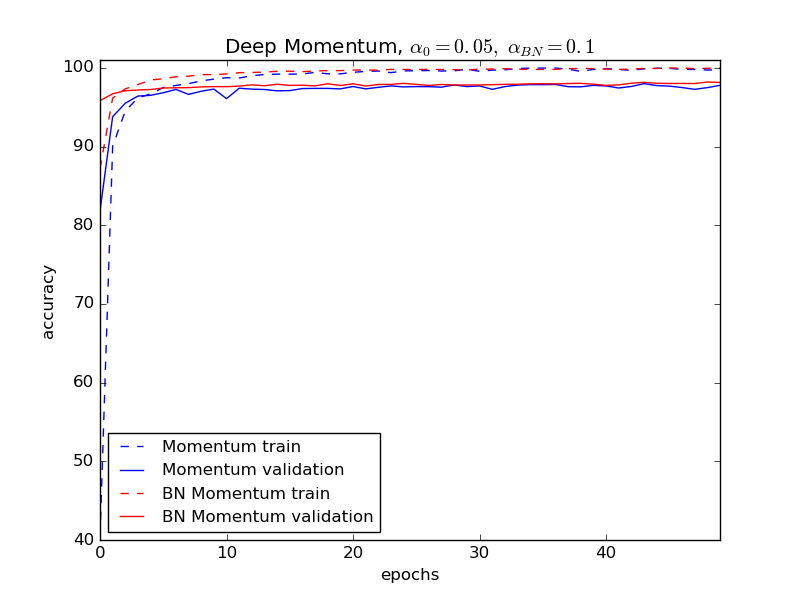
\includegraphics[scale=0.45]{images/mnistDeepMomentum1.png}
\caption{\small Моментум на глубокой сети, $10$ HL $\times 100$}
\end{minipage} \hfill
\begin{minipage}{0.45\textwidth}
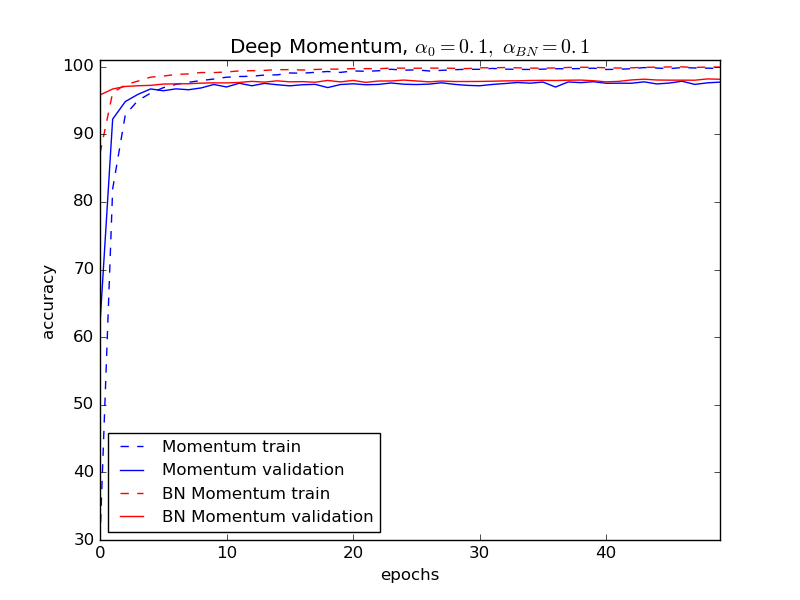
\includegraphics[scale=0.45]{images/mnistDeepMomentum2.png}
\caption{\small Моментум на глубокой сети, $10$ HL $\times 100$}
\end{minipage}
\end{figure}

\newpage


\begin{figure}[h!]
\centering
\begin{minipage}{0.45\textwidth}
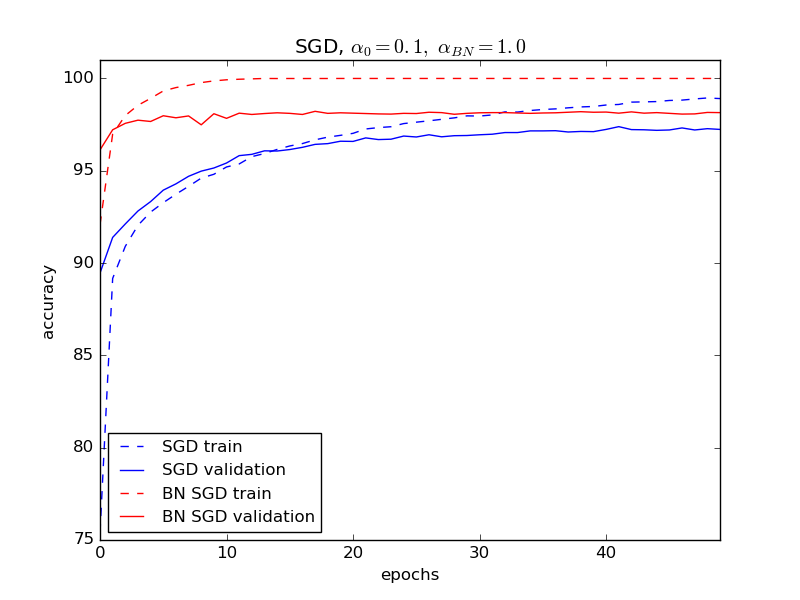
\includegraphics[scale=0.45]{images/mnistSGD1.png}
\caption{\small SGD на неглубокой сети, $3$ HL $\times 100$}
\end{minipage} \hfill
\begin{minipage}{0.45\textwidth}
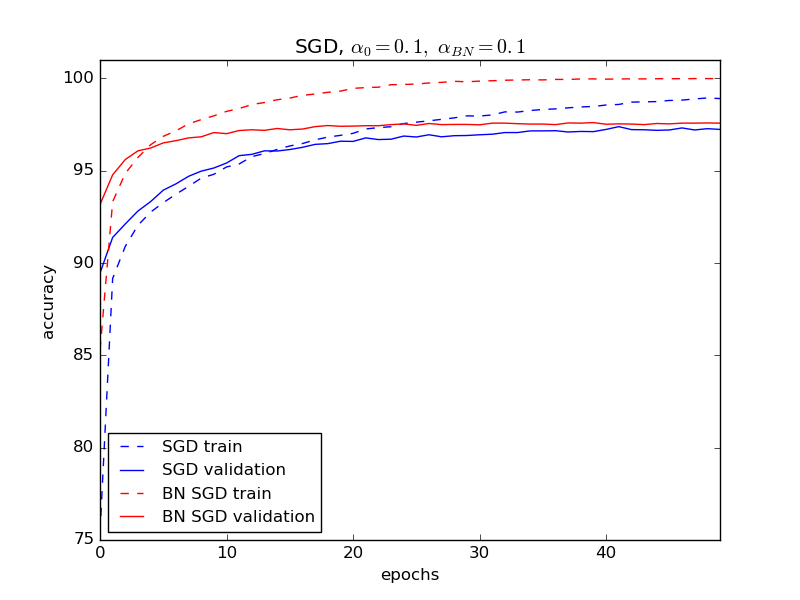
\includegraphics[scale=0.45]{images/mnistSGD2.png}
\caption{\small SGD на неглубокой сети, $3$ HL $\times 100$}
\end{minipage} \vfill
\begin{minipage}{0.45\textwidth}
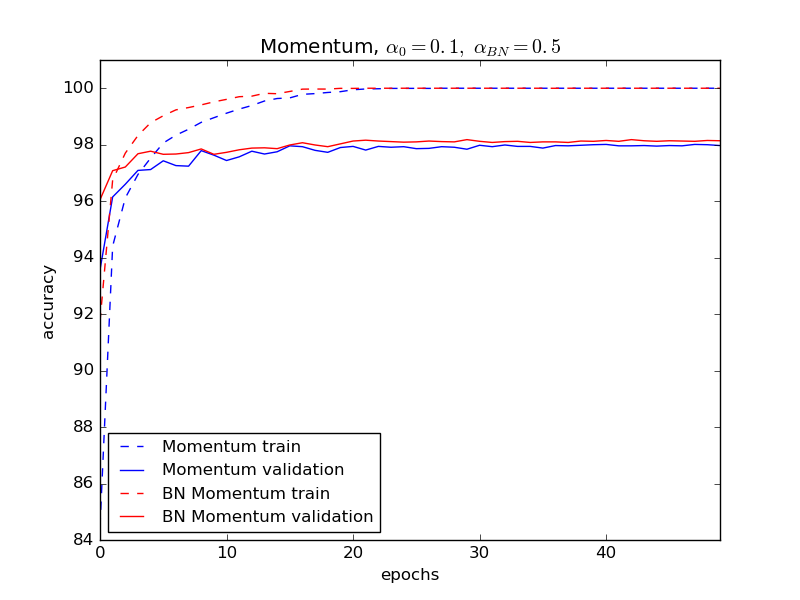
\includegraphics[scale=0.45]{images/mnistMomentum1.png}
\caption{\small Моментум на неглубокой сети, $3$ HL $\times 100$}
\end{minipage} \hfill
\begin{minipage}{0.45\textwidth}
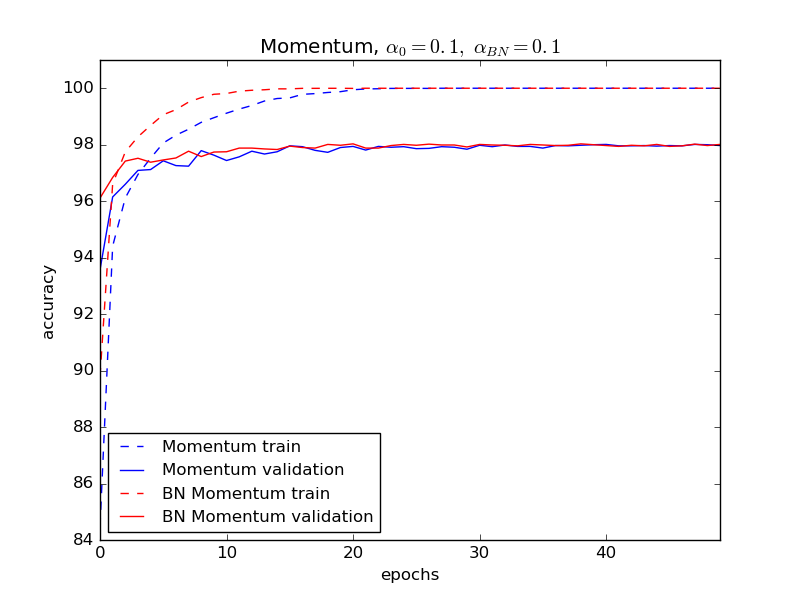
\includegraphics[scale=0.45]{images/mnistMomentum2.png}
\caption{\small Моментум на неглубокой сети, $3$ HL $\times 100$}
\end{minipage}
\end{figure}


Выводы:

\begin{enumerate}
\item батч-нормализация для Адам ведет себя более плавно при увеличении эпсилон;
\item батч-нормализация слабо улучшает Адам для обеих архитектур сети;
\item на глубокой сети SGD плохо обучается либо из-за плохо подобранного рейта, либо так и должно быть;
\item батч-нормализация так же слабо улучшает Моментум для обеих архитектур;
\end{enumerate}


\end{document}
